% !TEX root = doc.tex
% Copyright (c) 2017-2020 The ALF project.
% This is a part of the ALF project documentation.
% The ALF project documentation by the ALF contributors is licensed
% under a Creative Commons Attribution-ShareAlike 4.0 International License.
% For the licensing details of the documentation see license.CCBYSA.
%
%-----------------------------------------------------------------------------------
\subsection{Predefined lattices} \label{sec:predefined_lattices}
%-----------------------------------------------------------------------------------


The types \texttt{Lattice} and \texttt{Unit\_cell}, described in Section~\ref{sec:latt}, allow us to define arbitrary one- and two-dimensional Bravais lattices. The subroutine \texttt{Predefined\_Latt} provides some of the most common lattices, as described bellow.


\begin{figure}
        \begin{center}
                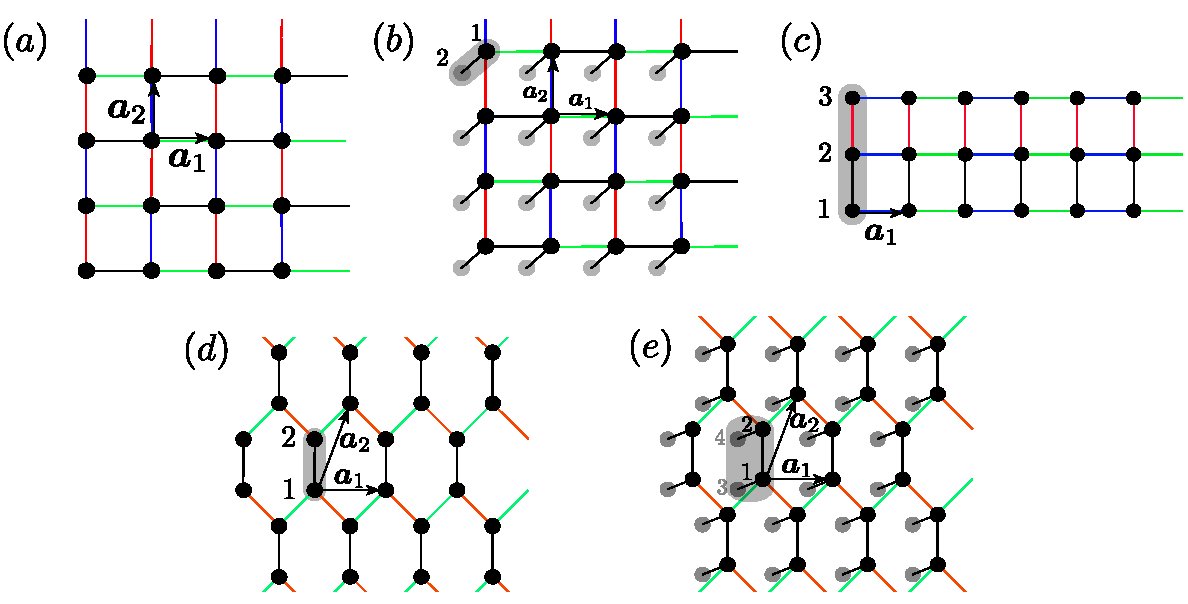
\includegraphics[width=\textwidth]{Figures/Lattices_all.pdf}
               
				
                \caption{Predefined lattices in ALF: (a) square, (b) bilayer square, (c) 3-leg ladder  (d) honeycomb and (e) bilayer honeycomb. Nontrivial unit cells are shown as gray regions, while gray sites belong to the second layer in bilayer systems.   The links between the orbitals denote the hopping matrix elements and we have assumed, for the purpose of the plot,  the absence of hopping in the second layer for bilayer systems. The color coding of the links denotes the checkerboard decomposition. }
                \label{fig_predefined_lattices}
        \end{center}
\end{figure}


The subroutine is called as:
\begin{lstlisting}[style=fortran]
Predefined_Latt(Lattice_type, L1, L2, Ndim, List, Invlist, Latt, Latt_Unit)
\end{lstlisting}
which returns a lattice of size \texttt{L1$\times$L2} of the given \texttt{Lattice\_type}, as detailed in Table~\ref{table:predefined_lattices}. Notice that the orbital position \texttt{Latt\_Unit\%Orb\_pos\_p(1,:)} is set to zero unless otherwise specified.
%
\begin{table}[h!]
	\begin{center}
	\begin{tabular}{@{} p{0.16\columnwidth}  p{0.12\columnwidth} p{0.09\columnwidth} p{0.54\columnwidth}  @{}}
		\toprule
		Argument                 & Type                & Role   & Description \\
		\midrule
		\texttt{Lattice\_type}   & \texttt{char}       & Input  & Lattice configuration, which can take the values:
		\vspace{-2\topsep} %sometimes dispensable
		\begin{itemize}
			\setlength{\itemsep}{0pt} \setlength{\parskip}{0pt} \setlength{\parsep}{0pt}
			\item[-] \texttt{Square}
			\item[-] \texttt{Honeycomb}
			\item[-] \texttt{Pi\_Flux}  (deprecated)
			\item[-] \texttt{N\_leg\_ladder}
			\item[-] \texttt{Bilayer\_square}
			\item[-] \texttt{Bilayer\_honeycomb}
			\vspace{-1.4\topsep} 
		\end{itemize} \\
	    %\vspace{-\topsep} \\ \vspace{-\topsep}
		\texttt{L1}, \texttt{L2} & \texttt{int}        & Input  & Lattice sizes (set \texttt{L2=1} for 1D lattices)\\
		\texttt{Ndim}            & \texttt{int}        & Output & Total number of orbitals\\
		\texttt{List}            & \texttt{int}        & Output & For every site index $\texttt{I} \in [1,\texttt{Ndim}]$, stores the corresponding lattice position, \texttt{List(I,1)}, and the (local) orbital index, \texttt{List(I,2)}\\
		\texttt{Invlist}         & \texttt{int}        & Output &  For every $\texttt{lattice\_position} \in [1,\texttt{Latt\%N}]$ and $\texttt{orbital} \in [1,\texttt{Norb}]$ stores the corresponding site index \texttt{I(lattice\_position,orbital)}\\
		\texttt{Latt}            & \texttt{Lattice}    & Output & Sets the lattice\\
		\texttt{Latt\_Unit}      & \texttt{Unit\_cell} & Output & Sets the unit cell\\
		\bottomrule
	\end{tabular}
\caption{Arguments of the subroutine \texttt{Predefined\_Latt}.   Note that the \texttt{Pi\_Flux} lattice is deprecated for the moment since it can be emulated with the Square lattice with half a flux quanta piercing each plaquette.}		\label{table:predefined_lattices}
\end{center}
\end{table}

In order to easily keep track of the orbital and unit cell, \texttt{List} and \texttt{Invlist} make use of a super-index, defined as shown below:
\begin{lstlisting}[style=fortran]
nc = 0                                  ! Super-index labeling unit cell and orbital
Do I = 1,Latt%N                         ! Unit-cell index 
   Do no = 1,Norb                       ! Orbital index
      nc = nc + 1
      List(nc,1) = I                    ! Unit-cell of super index nc
      List(nc,2) = no                   ! Orbital of super index nc
      Invlist(I,no) = nc                ! Super-index for given unit cell and orbital
   Enddo
Enddo
\end{lstlisting}
With the above lists one can run through all the orbitals and at each time keep track of the unit-cell and orbital index. We note that when translation symmetry is completely absent one can work with a single unit cell, and the number of orbitals will then correspond to the number of lattice sites. 

\subsubsection{Square lattice, Fig.~\ref{fig_predefined_lattices}(a)}

The choice \texttt{Lattice\_type = "Square"}  \index{\texttt{Square} } sets $\vec{a}_1 =  (1,0) $ and $\vec{a}_2 =  (0,1) $  and for an $L_1 \times L_2$  lattice  $\vec{L}_1 = L_1 \vec{a}_1$ and  $\vec{L}_2 = L_2 \vec{a}_2$:
\begin{lstlisting}[style=fortran]
Latt_Unit%N_coord   = 2
Latt_Unit%Norb      = 1
Latt_Unit%Orb_pos_p(1,:) = 0.d0 
a1_p(1) =  1.0  ; a1_p(2) =  0.d0
a2_p(1) =  0.0  ; a2_p(2) =  1.d0
L1_p    =  dble(L1)*a1_p
L2_p    =  dble(L2)*a2_p
Call Make_Lattice( L1_p, L2_p, a1_p,  a2_p, Latt )
\end{lstlisting}
Also, the number of orbitals per unit cell is given by \texttt{NORB=1} such that   $N_{\mathrm{dim}}   \equiv N_{\text{unit-cell}}   \cdot \texttt{NORB}  = \texttt{Latt\%N} \cdot \texttt{NORB}$, since $N_{\text{unit-cell}} = \texttt{Latt\%N}$.

\subsubsection{Bilayer Square lattice, Fig.~\ref{fig_predefined_lattices}(b)}
The "\texttt{Bilayer\_square}"  \index{\path{Bilayer_square}} configuration sets:
\begin{lstlisting}[style=fortran]
Latt_Unit%Norb     = 2
Latt_Unit%N_coord  = 2
do no = 1,2
   Latt_Unit%Orb_pos_p(no,1) = 0.d0 
   Latt_Unit%Orb_pos_p(no,2) = 0.d0 
   Latt_Unit%Orb_pos_p(no,3) = real(1-no,kind(0.d0))
enddo
Latt%a1_p(1) =  1.0  ; Latt%a1_p(2) =  0.d0
Latt%a2_p(1) =  0.0  ; Latt%a2_p(2) =  1.d0
Latt%L1_p    =  dble(L1)*a1_p
Latt%L2_p    =  dble(L2)*a2_p
Call Make_Lattice( L1_p, L2_p, a1_p,  a2_p, Latt )
\end{lstlisting}

\subsubsection{$N$-leg Ladder lattice,  Fig.~\ref{fig_predefined_lattices}(c)}
The "\texttt{N\_leg\_ladder}"  \index{\path{N_leg_ladder}} configuration sets:
\begin{lstlisting}[style=fortran]
Latt_Unit%Norb     = L2
Latt_Unit%N_coord  = 1
do no = 1,L2
   Latt_Unit%Orb_pos_p(no,1) = 0.d0 
   Latt_Unit%Orb_pos_p(no,2) = real(no-1,kind(0.d0))
enddo
a1_p(1) =  1.0   ; a1_p(2) =  0.d0
a2_p(1) =  0.0   ; a2_p(2) =  1.d0
L1_p    =  dble(L1)*a1_p
L2_p    =          a2_p
Call Make_Lattice( L1_p, L2_p, a1_p,  a2_p, Latt )
\end{lstlisting}



\subsubsection{Honeycomb lattice, Fig.~\ref{fig_predefined_lattices}(d)}

In order to carry out simulations on the Honeycomb lattice, which is a triangular Bravais lattice with two orbitals per unit cell, we choose \path{Lattice_type = "Honeycomb"}  \index{\path{Honeycomb}}, which sets
\begin{lstlisting}[style=fortran]
a1_p(1) =  1.D0   ; a1_p(2) =  0.d0
a2_p(1) =  0.5D0  ; a2_p(2) =  sqrt(3.D0)/2.D0
L1_p    =  Dble(L1) * a1_p
L2_p    =  dble(L2) * a2_p
Call Make_Lattice( L1_p, L2_p, a1_p,  a2_p, Latt )
Latt_Unit%Norb    = 2
Latt_Unit%N_coord = 3
Latt_Unit%Orb_pos_p(1,:) = 0.d0 
Latt_Unit%Orb_pos_p(2,:) = (a2_p(:) - 0.5D0*a1_p(:) ) * 2.D0/3.D0
\end{lstlisting}
The coordination number of this lattice is \texttt{ N\_coord=3 }  and  the number of orbitals per unit cell, \texttt{NORB=2}. The total number of orbitals is therefore \texttt{$N_{\mathrm{dim}}$=Latt\%N*NORB}.






\subsubsection{Bilayer Honeycomb lattice, Fig.~\ref{fig_predefined_lattices}(e)}
The "\texttt{Bilayer\_honeycomb}"  \index{\texttt{Bilayer\_honeycomb}} configuration sets:
\begin{lstlisting}[style=fortran]
Latt_Unit%Norb     = 4
Latt_Unit%N_coord  = 3
Latt_unit%Orb_pos_p = 0.d0
do n = 1,2
   Latt_Unit%Orb_pos_p(1,n) = 0.d0 
   Latt_Unit%Orb_pos_p(2,n) = (a2_p(n) - 0.5D0*a1_p(n) ) * 2.D0/3.D0
   Latt_Unit%Orb_pos_p(3,n) = 0.d0 
   Latt_Unit%Orb_pos_p(4,n) = (a2_p(n) - 0.5D0*a1_p(n) ) * 2.D0/3.D0
enddo
Latt_Unit%Orb_pos_p(3,3) = -1.d0
Latt_Unit%Orb_pos_p(4,3) = -1.d0
a1_p(1) =  1.D0   ; a1_p(2) =  0.d0
a2_p(1) =  0.5D0  ; a2_p(2) =  sqrt(3.D0)/2.D0
L1_p    =  dble(L1)*a1_p
L2_p    =  dble(L2)*a2_p
Call Make_Lattice( L1_p, L2_p, a1_p,  a2_p, Latt )
\end{lstlisting}

\subsubsection{$\pi$-Flux lattice (deprecated)}

The Pi\_Flux lattice has been deprecated, since it can be emulated with the Square lattice with half a flux quanta piercing each plaquette. Nonetheless, the configuration is still available, and sets:
\begin{lstlisting}[style=fortran]
Latt_Unit%Norb    = 2
Latt_Unit%N_coord = 4
a1_p(1) =  1.D0   ; a1_p(2) =   1.d0
a2_p(1) =  1.D0   ; a2_p(2) =  -1.d0
Latt_Unit%Orb_pos_p(1,:) = 0.d0 
Latt_Unit%Orb_pos_p(2,:) = (a1_p(:) - a2_p(:))/2.d0 
L1_p    =  dble(L1) * (a1_p - a2_p)/2.d0
L2_p    =  dble(L2) * (a1_p + a2_p)/2.d0
\end{lstlisting}


